% Cores dos gráficos: a mesma cor identifica o mesmo fluxo em todas as figuras
\definecolor{corNuvem}{HTML}{2A78D6}
\definecolor{corBorda}{HTML}{EB6834}
\definecolor{corFatias}{HTML}{008300}
\definecolor{corVotacao}{HTML}{6250D6}
\definecolor{corGrade}{HTML}{E1E0D9}
\definecolor{corEixo}{HTML}{898781}
\pgfplotsset{
    estiloResultados/.style={
        grid=major, grid style={color=corGrade, line width=0.3pt},
        axis x line*=bottom, axis y line*=left,
        axis line style={color=corEixo}, tick style={color=corEixo},
        tick label style={font=\scriptsize}, label style={font=\footnotesize},
        title style={font=\footnotesize},
        legend style={font=\scriptsize, draw=none, fill=white, fill opacity=0.85,
                      text opacity=1},
        legend cell align=left,
        /pgf/number format/use comma, /pgf/number format/1000 sep={.},
    },
}

Esta seção apresenta os resultados dos experimentos descritos na
Seção~\ref{sec:experimentos} e os analisa à luz das hipóteses da
Seção~\ref{subsec:hipotese}. Salvo indicação em contrário, os valores foram calculados a
partir dos dados brutos versionados no repositório do projeto, com os \textit{scripts} de
análise descritos naquela seção. A Seção~\ref{subsec:sintese_resultados} reúne o resultado
de cada hipótese, e a Seção~\ref{subsec:limitacoes_resultados}, as limitações que devem
acompanhar a sua leitura.

\subsection{Reconhecimento dos dígitos e efeito da quantização (H1)}
\label{subsec:resultado_h1}

A Tabela~\ref{tab:resultado_quantizacao} apresenta o desempenho do classificador de
dígitos. Nos 7.378 recortes de validação, o modelo em ponto flutuante acertou 7.043
(95,46\%) e o modelo em INT8, 7.037 (95,38\%): a quantização custou seis recortes, ou
0,08 ponto percentual.

\begin{table}[H]
    \centering
    \caption{Desempenho do classificador de dígitos em ponto flutuante e em INT8}
    \label{tab:resultado_quantizacao}
    \begin{tabularx}{\textwidth}{@{}>{\raggedright\arraybackslash}Xlrrr@{}}
        \toprule
        \textbf{Conjunto} & \textbf{Modelo} & \textbf{Leitura exata} & \textbf{Acerto por dígito} & \textbf{CER} \\
        \midrule
        Validação (7.378 recortes) & Ponto flutuante & --- & 95,46\% & --- \\
                                   & INT8            & --- & 95,38\% & --- \\
        \addlinespace
        Teste independente \textit{Word-Wheel} & INT8, fase A & 92,4\% & 97,3\% & 0,026 \\
        (1.894 imagens, 9.719 dígitos)          & INT8, fases A e B & 92,8\% & 97,7\% & 0,023 \\
        \bottomrule
    \end{tabularx}
    \legend{Fonte: Elaborado pelos autores (2026). Na validação, cada recorte é um único
    dígito, de modo que a acurácia por recorte coincide com o acerto por dígito.}
\end{table}

Como os dois modelos foram avaliados sobre os mesmos recortes, a comparação foi feita de
forma pareada. As duas versões deram a mesma resposta em 99,62\% dos recortes. Dos que
divergiram, 14 foram acertados apenas pelo modelo em ponto flutuante e 8 apenas pelo modelo
INT8. Pelo teste exato de McNemar, que considera apenas esses pares discordantes, a
diferença não é estatisticamente significativa ($p = 0{,}29$). A ordem de grandeza da perda
também aparece em outro detalhe: executado com os \textit{kernels} otimizados XNNPACK, em
vez dos \textit{kernels} sem esse delegado usados no restante do trabalho, o mesmo arquivo
INT8 acertou 7.040 recortes. A troca da implementação dos operadores altera o resultado na
mesma escala que a própria quantização.

O resultado é coerente com o tamanho e a forma do modelo. A quantização completa após o
treinamento, calibrada com um conjunto representativo, foi suficiente para um classificador
convolucional pequeno, com ativações ReLU, e o pipeline B não precisou do treinamento
consciente da quantização descrito na Seção~\ref{sec:fundamentos}, que no pipeline A havia
sido usado justamente para mitigar a degradação \cite{ferreira2022compressao}. Os dois
modelos INT8 somam 93,3~KB (81,5~KB do classificador e 11,8~KB da localização), na faixa de
centenas de quilobytes relatada para modelos de \gls{ocr} de medidores em hardware
embarcado \cite{ademola2023resource, jawas2018water}.

Por classe, a acurácia em INT8 variou de 90,84\% no dígito 7 a 97,21\% no dígito 0, que é
também o mais frequente. Os dígitos 7, 9 e 6 foram os mais difíceis (90,84\%, 91,64\% e
92,18\%). Dos 341 erros, 110 (32\%) foram classificações como 0, o que indica que os pesos
por classe compensaram apenas em parte o excesso de zeros no treino.

No teste independente, com as 1.894 imagens que ficaram fora de todo o treinamento, o
modelo INT8 leu 92,8\% das leituras inteiras e 97,7\% dos dígitos, com CER de 0,023. O
ajuste fino com as imagens do \gls{esp32cam} (fase B) não prejudicou a generalização:
melhorou 0,4 ponto percentual a leitura exata em relação ao modelo da fase A. Esse número
é inferior aos 95,6\% de leituras exatas que uma versão anterior do classificador obtinha
nesse mesmo conjunto, mas aquela versão havia sido treinada com essas imagens. A diferença
mostra o quanto um teste contaminado pelo treino superestima o desempenho, e é por isso que
o valor adotado é o do teste independente.

Quanto à hipótese H1, o modelo INT8 teve, de fato, acurácia menor que a do modelo em ponto
flutuante, como previsto. A redução, porém, é de 0,08 ponto percentual e não é
estatisticamente significativa, de modo que, na prática, a quantização não penalizou o
reconhecimento. Além disso, como os dois fluxos executam os mesmos modelos INT8
(Seção~\ref{subsec:visao_geral}), a acurácia não é um fator de diferença entre eles: o
servidor poderia executar o modelo em ponto flutuante sem restrição de memória, mas
ganharia no máximo essa mesma fração.

\subsection{Leitura de ponta a ponta}
\label{subsec:resultado_leitura}

A Tabela~\ref{tab:resultado_leitura} apresenta a leitura completa, da imagem da câmera até a
sequência de dígitos, nas configurações descritas na Seção~\ref{subsubsec:exp_leitura}.

\begin{table}[H]
    \centering
    \caption{Leitura de ponta a ponta nos dois fluxos}
    \label{tab:resultado_leitura}
    \begin{tabularx}{\textwidth}{@{}>{\raggedright\arraybackslash}X>{\raggedright\arraybackslash}p{3.4cm}rrrr@{}}
        \toprule
        & & \multicolumn{2}{c}{\textbf{Fluxo em borda}} & \multicolumn{2}{c}{\textbf{Fluxo em nuvem}} \\
        \cmidrule(lr){3-4}\cmidrule(l){5-6}
        \textbf{Conjunto} & \textbf{Janela de dígitos} & \textbf{Leituras} & \textbf{Dígitos} & \textbf{Leituras} & \textbf{Dígitos} \\
        \midrule
        \multirow{3}{=}{Comum (39 fotos, 222 dígitos)}
                         & Prevista pelo modelo & 0\% & 15\% & 0\% & 16\% \\
                         & Marcada à mão        & 46\% & 85\% & 46\% & 85\% \\
                         & Marcada à mão, quadro endireitado & --- & --- & 82\% & 92\% \\
        \addlinespace
        \multirow{3}{=}{Físico (21 fotos, 152 dígitos)}
                         & Prevista pelo modelo & 10\% & 31\% & 0\% & 27\% \\
                         & Marcada à mão, quadro endireitado & 10\% & 36\% & 10\% & 37\% \\
                         & Marcada à mão, endireitado, tons invertidos no fundo escuro & 14\% & 56\% & 14\% & 56\% \\
        \bottomrule
    \end{tabularx}
    \legend{Fonte: Elaborado pelos autores (2026). Leituras: taxa de leitura exata;
    dígitos: acerto por dígito. No conjunto comum, a inclinação é estimada pela transformada
    de Hough e só é corrigida no servidor; no físico, é marcada à mão e corrigida nos dois
    fluxos.}
\end{table}

\subsubsection{O gargalo é a localização da janela}

Com a janela prevista pelo modelo de localização, nenhuma das 39 fotos do conjunto comum
foi lida corretamente, em nenhum dos dois fluxos, e apenas 15\% a 16\% dos dígitos
coincidiram com o gabarito. Esse resultado
\textbf{não mede o classificador}. Nesse conjunto, a máscara prevista teve Dice de 0,23 e
IoU de 0,13 em relação à janela real, valores ainda menores que os do teste do próprio
modelo (Seção~\ref{subsubsec:segmentacao}), e a caixa prevista teve mediana de
$130 \times 90$ pixels, contra cerca de $97 \times 18$ pixels da janela real. Com uma caixa
que cobre quase todo o mostrador, as fatias não correspondem aos roletes. Endireitar o
quadro no servidor antes da localização também não resolveu: a caixa continuou com cerca de
90 pixels de altura, e a leitura exata continuou em 0\%.

Quando a janela é marcada à mão, o mesmo classificador, com o mesmo fatiamento, leu 46\%
das leituras e 85\% dos dígitos; com o quadro endireitado pelo servidor, chegou a 82\% das
leituras e 92\% dos dígitos. No medidor de seis roletes, com 27 fotos, foram 85\% das
leituras e 97\% dos dígitos. A diferença entre 0\% e 82\% vem inteiramente da janela: o
modelo de reconhecimento é o mesmo nas duas linhas. As sete leituras que ainda falharam
nessa configuração são as três fotos de uma mesma leitura com contraste muito baixo e
quatro fotos de duas leituras do medidor de seis roletes, cada uma com um ou dois dígitos
trocados.

Esse comportamento se repetiu no hardware. Nas primeiras capturas do firmware de
depuração, antes do ajuste da posição da câmera, a caixa prevista era enorme e a leitura,
errada.
Depois que a câmera foi posicionada à mão, de modo que a janela ocupasse a maior parte do
quadro, a caixa encolheu, e as doze últimas capturas leram a leitura real do medidor de
teste, \texttt{046663}. Nas cinco capturas do \gls{esp32cam} com a janela marcada à mão
(Figura~\ref{fig:leitura_caixa_manual}), todas as leituras e os 26 dígitos foram
reconhecidos.

\subsubsection{A compressão JPEG não afeta a leitura}

Com a janela marcada à mão, os dois fluxos tiveram exatamente o mesmo número de leituras
exatas (18 de 39) e de dígitos corretos (189 de 222). A compressão JPEG com qualidade 90,
que o fluxo em nuvem aplica antes da transmissão, não alterou a leitura. Com a janela
prevista pelo modelo, por outro lado, os dois fluxos deram a mesma leitura em apenas 10 das
39 fotos: pequenas diferenças introduzidas pela compressão mudam a máscara prevista e, com
ela, a caixa. A compressão afeta o modelo de localização, que já falha, e não o
classificador.

\subsubsection{Precisão exigida da ROI}

Como a solução adotada substitui a localização automática por uma ROI calibrada na
instalação, a Figura~\ref{fig:tolerancia_roi} mostra quanto erro de posição a leitura
tolera. Sem erro, a leitura exata é de 82\% com fatias iguais e de 87\% com a votação entre
cinco caixas deslocadas. Com até 2~pixels de erro em cada coordenada, cai para 62\% e 70\%;
com até 6~pixels, para 20\% e 26\%. Como cada dígito tem cerca de 16~pixels de largura no
quadro de $160 \times 120$ pixels, um erro de 2~pixels já corresponde a um oitavo de dígito.
A votação compensa cerca de 1~pixel de erro: com ela, a leitura com $\pm$2~pixels fica
próxima da leitura sem votação com $\pm$1~pixel. O custo é executar o classificador cinco
vezes.

\begin{figure}[H]
    \centering
    \caption{Leitura exata em função do erro de posição da ROI}
    \label{fig:tolerancia_roi}
    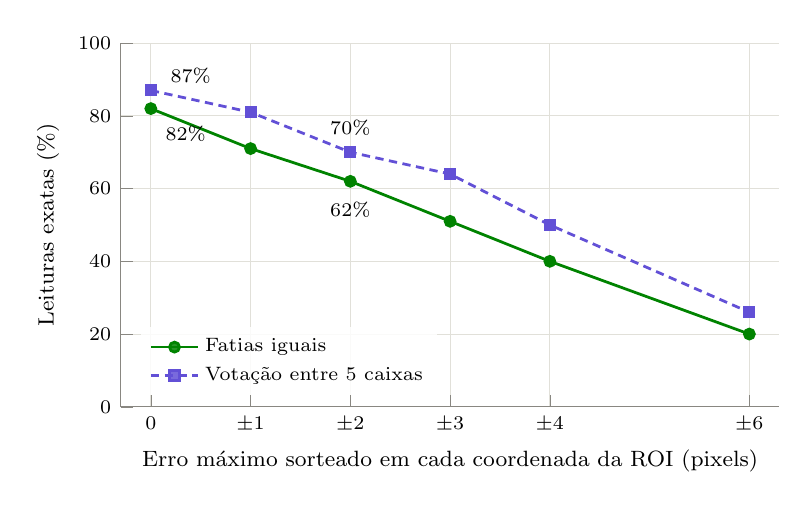
\begin{tikzpicture}
        \begin{axis}[
            estiloResultados,
            width=0.82\textwidth, height=6.2cm,
            xmin=-0.3, xmax=6.3, ymin=0, ymax=100,
            xtick={0,1,2,3,4,6}, xticklabels={0,$\pm$1,$\pm$2,$\pm$3,$\pm$4,$\pm$6},
            ytick={0,20,40,60,80,100},
            xlabel={Erro máximo sorteado em cada coordenada da ROI (pixels)},
            ylabel={Leituras exatas (\%)},
            legend pos=south west,
        ]
            \addplot[color=corFatias, line width=1pt, mark=*, mark size=1.8pt]
                coordinates {(0,82) (1,71) (2,62) (3,51) (4,40) (6,20)};
            \addlegendentry{Fatias iguais}
            \addplot[color=corVotacao, line width=1pt, mark=square*, mark size=1.7pt,
                     densely dashed, mark options={solid}]
                coordinates {(0,87) (1,81) (2,70) (3,64) (4,50) (6,26)};
            \addlegendentry{Votação entre 5 caixas}
            \node[font=\scriptsize, color=black, anchor=west] at (axis cs:0.1,91) {87\%};
            \node[font=\scriptsize, color=black, anchor=north west] at (axis cs:0.05,80) {82\%};
            \node[font=\scriptsize, color=black, anchor=south] at (axis cs:2,72) {70\%};
            \node[font=\scriptsize, color=black, anchor=north] at (axis cs:2,59) {62\%};
        \end{axis}
    \end{tikzpicture}
    \legend{Fonte: Elaborado pelos autores (2026). Conjunto comum, fluxo em nuvem, quadro
    endireitado; média de três sorteios do erro.}
\end{figure}

Calibrar a ROI com uma única leitura e aplicá-la às demais fotos do mesmo medidor rendeu
apenas 26\% a 30\% das leituras no medidor de seis roletes e 0\% no de cinco. Esse cenário,
porém, é pessimista: as fotos do conjunto comum são de um monitor cujo zoom e cuja posição
mudaram entre leituras, o que deslocou a janela em 3,5 a 5~pixels, em média, no primeiro
medidor e em 12 a 18~pixels no segundo. Os valores confirmam que a precisão da calibração é
o fator que decide a leitura: em uma instalação com a câmera fixada mecanicamente, espera-se
que a janela não se desloque entre leituras, mas essa condição não foi testada.

\subsubsection{Hidrômetros físicos}

No conjunto de hidrômetros físicos, com a janela prevista pelo modelo, o fluxo em borda
leu 2 das 21 fotos e o fluxo em nuvem, nenhuma, com 27\% a 31\% dos dígitos corretos. As
duas leituras corretas são de fotos em que a janela de dígitos ocupa a maior parte do
quadro, a mesma condição em que a caixa prevista se aproximou da janela no firmware de
depuração.

Com a janela e a inclinação marcadas à mão, porém, o resultado mudou pouco: 2 das 21
leituras e 36\% a 37\% dos dígitos, nos dois fluxos. Ao contrário do conjunto comum,
portanto, nos medidores reais a localização da janela não é a única causa dos erros. A
Tabela~\ref{tab:resultado_fisico_polaridade} separa as fotos pela polaridade da janela e
mostra de onde eles vêm.

\begin{table}[H]
    \centering
    \caption{Leitura do conjunto físico com a janela marcada à mão, por polaridade da janela}
    \label{tab:resultado_fisico_polaridade}
    \begin{tabularx}{\textwidth}{@{}>{\raggedright\arraybackslash}Xcrrrr@{}}
        \toprule
        & & \multicolumn{2}{c}{\textbf{Tons originais}} & \multicolumn{2}{c}{\textbf{Tons invertidos}} \\
        \cmidrule(lr){3-4}\cmidrule(l){5-6}
        \textbf{Fotos} & \textbf{Qtd.} & \textbf{Leituras} & \textbf{Dígitos} & \textbf{Leituras} & \textbf{Dígitos} \\
        \midrule
        Dígitos escuros em fundo claro, fotos frontais & 7 & 2 & 43/48 & --- & --- \\
        Dígitos escuros em fundo claro, perspectiva extrema & 2 & 0 & 2/10 & --- & --- \\
        Dígitos claros em fundo escuro & 12 & 0 & 11/94 & 1 & 40/94 \\
        \bottomrule
    \end{tabularx}
    \legend{Fonte: Elaborado pelos autores (2026). Fluxo em nuvem; leituras: número de
    leituras exatas. A inversão só se aplica às fotos de fundo escuro.}
\end{table}

Nas sete fotos frontais de medidores com dígitos escuros em fundo claro, o classificador
acertou 43 dos 48 dígitos (90\%), resultado próximo ao do conjunto comum, e duas fotos foram
lidas por inteiro; dos cinco dígitos errados, três estão no último rolete, parado entre dois
números. Nas duas fotos com perspectiva extrema, em que os dígitos aparecem inclinados em
relação às fatias, a leitura falhou.

Nas 12 fotos de medidores com dígitos claros em fundo escuro, o classificador respondeu 0
na maior parte das fatias e acertou apenas 11 dos 94 dígitos (12\%). A causa está no
treino: considerando de fundo escuro os recortes cuja mediana dos pixels fica abaixo de 100,
apenas 421 dos 49.038 recortes de treino (0,9\%) têm essa polaridade, e o modelo responde
com a classe mais frequente. Invertendo os tons da janela nessas fotos, o que equivale a
informar a polaridade do medidor na instalação, assim como o número de roletes, o acerto
subiu para 40 dos 94 dígitos (43\%), e uma foto passou a ser lida por inteiro. As fotos que
continuaram com erros têm perspectiva forte, reflexos no vidro, baixo contraste, dígitos com
cerca de 10 pixels de largura ou a janela cortada pela borda do quadro. A votação entre
caixas deslocadas não melhorou o resultado.

Com a janela, a inclinação e a polaridade informadas, o conjunto físico chegou a 3 das 21
leituras (14\%) e 56\% dos dígitos. Os erros que restam, porém, não têm todos a mesma
origem, e a maior parte não está no fluxo nem na janela. A
Tabela~\ref{tab:causas_erros_fisico} classifica as fotos pela causa dos erros.

\begin{table}[H]
    \centering
    \caption{Causas dos erros de leitura no conjunto físico}
    \label{tab:causas_erros_fisico}
    \begin{tabularx}{\textwidth}{@{}l>{\raggedright\arraybackslash}X>{\raggedright\arraybackslash}p{4.2cm}@{}}
        \toprule
        \textbf{Origem} & \textbf{Causa} & \textbf{Fotos} \\
        \midrule
        Captura & Perspectiva extrema, com os dígitos inclinados em relação às fatias & 01, 06, 11, 21, 26 \\
        Captura & Janela cortada pela borda do quadro & 21, 23, 25 \\
        Captura & Reflexo no vidro, baixo contraste ou dígitos com cerca de 10 pixels de largura & 02, 05, 15, 16 \\
        \addlinespace
        Treino & Dígitos claros em fundo escuro & 02, 03, 05, 06, 07, 11, 13, 15, 16, 21, 23, 24 \\
        Treino & Último rolete parado entre dois números & 04, 20, 25 \\
        \addlinespace
        Classificador & Dígito visível lido como 0 & 08, 22 \\
        \bottomrule
    \end{tabularx}
    \legend{Fonte: Elaborado pelos autores (2026). Uma foto pode ter mais de uma causa. As
    fotos 12 e 19 foram lidas sem erro com a janela marcada à mão.}
\end{table}

As causas de captura são resolvidas por uma instalação adequada, com a câmera de frente para
o medidor e a janela inteira no quadro, e não indicam falha do \gls{ocr}. As causas de
treino, ao contrário, são limitações do classificador, e não das fotos. A foto 07, por
exemplo, é frontal e nítida, mas foi lida como \texttt{00000000} com os tons originais e por
inteiro com os tons invertidos. O rolete parado entre dois números, por sua vez, ocorre em
qualquer medidor em uso, mas as imagens com essa situação foram descartadas do principal
conjunto de treino por terem rótulo ambíguo (Seção~\ref{subsubsec:dados_ocr}). Restam, por
fim, erros do próprio classificador em dígitos visíveis, raros nas fotos de boa qualidade.

Para estimar o desempenho em uma instalação adequada, foram separadas as fotos que atendem a
três condições: câmera frontal, sem perspectiva extrema; dígitos escuros em fundo claro, a
polaridade do treino; e todos os dígitos visíveis no quadro. Restaram seis fotos (04, 08,
12, 19, 20 e 22), com 41 dígitos. Com a janela marcada à mão, o classificador acertou 37 dos
41 dígitos (90,2\%, com intervalo de confiança de 95\% de 77,5\% a 96,1\%) e leu por
inteiro duas das seis fotos, nos dois fluxos; com a janela prevista pelo modelo, o acerto foi
de 61\% a 66\% dos dígitos. Dos quatro dígitos errados, dois estão no último rolete, parado
entre dois números, e dois são dígitos visíveis lidos como 0. Esse subconjunto foi definido
depois da avaliação do conjunto completo e é pequeno, de modo que deve ser lido como uma
indicação do que uma instalação adequada permite, e não como substituto do resultado das 21
fotos.

Os resultados do conjunto físico indicam, portanto, o que uma instalação real precisa:
câmera frontal com a janela inteira no quadro; ROI, inclinação e polaridade calibradas; e um
classificador treinado também com dígitos claros em fundo escuro, por exemplo pela inversão
dos recortes no aumento de dados, e com roletes em transição.

Em síntese, os resultados próximos de zero obtidos com a janela prevista pelo modelo são
causados pela localização automática, e não pelo classificador nem pelo fluxo: com a janela
informada, a leitura chega a 82\% das leituras e 92\% dos dígitos no conjunto comum e a
90\% dos dígitos nas fotos de medidores reais que atendem às condições de instalação, e o
classificador reconhece 97,7\% dos dígitos de um conjunto público independente. Em
medidores reais, porém, a janela correta não basta: a geometria da captura, que a instalação
resolve, e as limitações do treino quanto à polaridade e aos roletes em transição também
limitam a leitura. Como os dois fluxos executam o mesmo pipeline e a compressão não altera a
leitura, essas conclusões valem igualmente para a borda e para a nuvem.

\subsection{Latência (H2)}
\label{subsec:resultado_latencia}

A Tabela~\ref{tab:resultado_latencia} apresenta a latência ponta a ponta dos dois fluxos,
medida com o nó no modo autônomo.

\begin{table}[H]
    \centering
    \caption{Latência ponta a ponta dos dois fluxos}
    \label{tab:resultado_latencia}
    \begin{tabularx}{\textwidth}{@{}Xrr@{}}
        \toprule
        \textbf{Marco, desde o disparo} & \textbf{Fluxo em nuvem} & \textbf{Fluxo em borda} \\
        \midrule
        Captura concluída & 0,70~s & --- \\
        Leitura pronta no nó & --- & 18,20~s \\
        Primeiro pacote no computador & 1,97~s & 18,84~s \\
        \textbf{Dado disponível no servidor (mediana)} & \textbf{189,1~s} & \textbf{18,84~s} \\
        Mínimo e máximo & 172,7 a 213,5~s & 18,836 a 18,840~s \\
        Desvio-padrão & 11,8~s & 0,9~ms \\
        Leituras consideradas & 20 imagens completas & 27 leituras recebidas \\
        \bottomrule
    \end{tabularx}
    \legend{Fonte: Elaborado pelos autores (2026).}
\end{table}

A latência do fluxo em borda foi de 18,84~s, cerca de dez vezes menor que os 189,1~s do
fluxo em nuvem. Na corrida controlada, com o nó sempre ligado, a latência do fluxo em nuvem
foi de 197,1~s (de 148,1 a 204,9~s, com 21 imagens completas), compatível com a corrida em
modo autônomo, já que as imagens dessa corrida foram maiores (mediana de 4.379 contra
4.068~bytes).

Os dois fluxos têm gargalos opostos. No fluxo em nuvem, a imagem fica pronta em 0,70~s, e
quase toda a latência é a transmissão. Cada bloco leva cerca de 8,1~s: os 7~s do intervalo
entre pacotes e cerca de 1,1~s de comando AT, transmissão e confirmação do módulo. Por isso,
a latência cresce com o tamanho do JPEG: as três imagens mais rápidas tinham 22 blocos e
chegaram em cerca de 173~s, e a mais lenta, com 27 blocos, em 213,5~s. O tempo no ar
propriamente dito, de cerca de 3~s por imagem (Tabela~\ref{tab:tempo_no_ar}), representa
menos de 2\% da latência. Em 3 das 30 leituras, o primeiro bloco só chegou entre 10 e 12~s
após o disparo, o que indica que o bloco inicial se perdeu. A execução do \gls{ocr} no servidor, que
não está incluída na medição, leva cerca de 6~ms (Tabela~\ref{tab:tempo_inferencia}) e não
altera esses números.

No fluxo em borda, ao contrário, quase toda a latência é processamento. A leitura fica
pronta no nó em 18,20~s, dos quais cerca de 15,5~s são a localização da janela e 2,0~s a
classificação dos dígitos, segundo o log do próprio firmware; o envio e a recepção levam
mais 0,64~s. Como nenhum desses passos depende da rede, a latência é praticamente
determinística, com desvio-padrão de 0,9~ms.

Dois cenários ajudam a avaliar se a conclusão depende das escolhas de implementação. Ambos
são estimativas, e não medições. No fluxo em borda, retirar a localização da janela, como
prevê a solução com ROI calibrada, reduziria a latência para cerca de 3,3~s. No fluxo em
nuvem, mesmo eliminando o intervalo de 7~s entre pacotes, que é uma escolha conservadora e
não uma exigência regulatória (Seção~\ref{subsubsec:formato_mensagens}), restaria cerca de
1,1~s por bloco, ou aproximadamente 26~s para uma imagem de 24 blocos, acima da latência
medida no fluxo em borda. Assim, a vantagem do processamento local em latência não depende
do intervalo escolhido.

Quanto à latência, a hipótese H2 foi confirmada com folga, em concordância com a menor
latência atribuída à computação em borda na
Tabela~\ref{tab:vant_desvant_edge_cloud} \cite{andriulo2024edge}. Nesta implementação, a
vantagem vem da quantidade de dados transmitida, e não da velocidade do processamento: o
microcontrolador é cerca de 2.800 vezes mais lento que o servidor na inferência, mas o
fluxo em borda transmite 9~bytes por leitura, contra cerca de 4~KB do fluxo em nuvem.

\subsection{Entrega dos dados (H2)}
\label{subsec:resultado_entrega}

A Tabela~\ref{tab:resultado_entrega} apresenta a entrega dos dados nas três corridas, por
pacote e por leitura.

\begin{table}[H]
    \centering
    \caption{Entrega por pacote e por leitura}
    \label{tab:resultado_entrega}
    \begin{tabularx}{\textwidth}{@{}Xrr@{}}
        \toprule
        \textbf{Corrida} & \textbf{\gls{pdr} por pacote} & \textbf{Entrega por leitura} \\
        \midrule
        Fluxo em nuvem, modo autônomo & 699/713 (98,0\%) & 20/30 (66,7\%) \\
        Fluxo em nuvem, modo controlado & 749/759 (98,7\%) & 21/30 (70,0\%) \\
        Fluxo em borda, modo autônomo & 27/34 (79,4\%) & 27/34 (79,4\%) \\
        \bottomrule
    \end{tabularx}
    \legend{Fonte: Elaborado pelos autores (2026).}
\end{table}

As duas métricas apontam em sentidos opostos. Por pacote, o fluxo em nuvem entregou mais:
98,0\% contra 79,4\%, diferença estatisticamente significativa (teste exato de Fisher,
$p < 0{,}001$). Por leitura, o fluxo em borda entregou mais: 79,4\% contra 66,7\%; com 30 e
34 leituras, porém, essa diferença não é estatisticamente significativa ($p = 0{,}27$), nem
em relação à corrida controlada ($p = 0{,}40$).

No fluxo em nuvem, a diferença entre as duas métricas decorre da fragmentação. Como nenhum
dos firmwares retransmite blocos no modo autônomo, basta um bloco perdido para que a imagem
não seja remontada: as dez imagens incompletas da corrida em modo autônomo perderam apenas
um ou dois blocos cada. Se cada bloco fosse perdido de forma independente, com a taxa
observada, seriam esperadas 18,7 imagens completas em 30, e foram obtidas 20; na corrida
controlada, 21,5 esperadas e 21 obtidas. Ou seja, a probabilidade de uma imagem chegar
inteira é aproximadamente o \gls{pdr} elevado ao número de blocos, e uma taxa de 98\% por
pacote resulta em pouco mais de 60\% das imagens de 24 blocos. A retransmissão seletiva dos
blocos perdidos recuperaria essas leituras, mas com tempo no ar e energia adicionais, e não
foi implementada no modo autônomo.

No fluxo em borda, as perdas não se explicam pelo sinal: o RSSI ficou entre $-31$ e
$-27$~dBm, e, nos dois ciclos perdidos registrados no log do nó, o módulo aceitou o envio
sem falhas. As perdas também não se distribuíram de maneira uniforme no fluxo em nuvem. Na
corrida controlada, 6 dos 10 blocos perdidos foram o primeiro ou o último de uma imagem,
embora esses blocos sejam apenas 60 dos 759 enviados: uma taxa de perda de 10\% nas
extremidades de cada sequência, contra 0,57\% nos blocos do meio (teste exato de Fisher,
$p < 0{,}001$). O \textit{uplink} do fluxo em borda é, ao mesmo tempo, o primeiro e o último
da sua sequência, e a sua taxa de perda, de 20,6\%, não difere significativamente da taxa
das extremidades ($p = 0{,}21$). A causa não foi investigada; a coincidência sugere que as
perdas estão associadas ao início e ao fim de uma sequência de transmissões, no módulo ou no
receptor de canal único, e não ao enlace de rádio.

Quanto à entrega, portanto, a hipótese H2 não foi confirmada: o fluxo em borda entregou
mais leituras, mas sem significância estatística, e entregou uma fração menor de pacotes.
O resultado mostra ainda que a métrica de interesse da aplicação é a entrega por leitura, e
não o \gls{pdr}: um \gls{pdr} de 98\% por pacote resultou em um terço das imagens perdidas.
Em um cenário com retransmissão, a diferença de custo seria grande: o fluxo em borda
reenviaria um pacote de 9~bytes, enquanto o fluxo em nuvem precisaria reenviar os blocos
faltantes e manter o nó acordado durante a espera.

\subsection{Consumo de energia e autonomia (H3)}
\label{subsec:resultado_energia}

A Figura~\ref{fig:corrente_ciclos} mostra a corrente do nó durante um ciclo típico de cada
fluxo, e a Tabela~\ref{tab:resultado_energia} resume as medições.

\begin{figure}[H]
    \centering
    \caption{Corrente do nó sensor em um ciclo de leitura de cada fluxo}
    \label{fig:corrente_ciclos}
    \begin{tikzpicture}
        \begin{groupplot}[
            estiloResultados,
            group style={group size=1 by 2, vertical sep=13mm},
            width=\textwidth, height=5cm,
            xmin=0, xmax=225, ymin=0, ymax=250,
            ytick={0,50,100,150,200,250},
            ylabel={Corrente (mA)},
        ]
            \nextgroupplot[title={(a) Fluxo em nuvem: ciclo de 219~s e 4,65~mAh}]
            \addplot[color=corNuvem, line width=0.35pt] table {sections/dados/corrente_ciclo_nuvem.dat};
            \node[font=\scriptsize, anchor=south] at (axis cs:95,212) {picos de transmissão, um por bloco};
            \node[font=\scriptsize, anchor=north] at (axis cs:95,72) {espera entre blocos, $\approx$80~mA};
            \node[font=\scriptsize, anchor=south] at (axis cs:205,30) {repouso};

            \nextgroupplot[title={(b) Fluxo em borda: ciclo de 49~s e 0,82~mAh},
                           xlabel={Tempo desde o despertar (s)}]
            \addplot[color=corBorda, line width=0.35pt] table {sections/dados/corrente_ciclo_borda.dat};
            \draw[-{Stealth[length=1.5mm]}, color=black!70, line width=0.4pt] (axis cs:57,114) -- (axis cs:22,114);
            \node[font=\scriptsize, anchor=west] at (axis cs:58,114) {inferência, $\approx$114~mA};
            \node[font=\scriptsize, anchor=south west] at (axis cs:21,212) {\textit{uplink}};
            \node[font=\scriptsize, anchor=west] at (axis cs:52,25) {repouso, $\approx$25~mA};
        \end{groupplot}
    \end{tikzpicture}
    \legend{Fonte: Elaborado pelos autores (2026). Ciclos com carga próxima da mediana de
    cada corrida; envelope dos valores mínimo e máximo a cada 0,25~s das amostras de 100~Hz.}
\end{figure}

\begin{table}[H]
    \centering
    \caption{Consumo do nó sensor por ciclo de leitura, com repouso de 30~s}
    \label{tab:resultado_energia}
    \begin{tabularx}{\textwidth}{@{}Xrr@{}}
        \toprule
        \textbf{Grandeza} & \textbf{Fluxo em nuvem} & \textbf{Fluxo em borda} \\
        \midrule
        Ciclos medidos & 30 & 32 \\
        \textbf{Carga por leitura (média)} & \textbf{4,64~mAh} & \textbf{0,824~mAh} \\
        Desvio-padrão da carga & 0,24~mAh & 0,014~mAh \\
        Carga apenas do tempo acordado & 4,46~mAh & 0,62~mAh \\
        Tempo acordado & 189,9~s (173 a 219~s) & 19,45~s \\
        Corrente média acordado & 84,5~mA & 114~mA \\
        Picos de transmissão & 207 a 220~mA & 206 a 227~mA \\
        Corrente em repouso & 23,7~mA & 25,2~mA \\
        Período do ciclo & 218,5~s & 49,1~s \\
        \bottomrule
    \end{tabularx}
    \legend{Fonte: Elaborado pelos autores (2026). No fluxo em borda, tempo acordado e
    corrente acordado são medianas; três ciclos tiveram a fronteira deslocada por picos
    isolados de uma amostra.}
\end{table}

Uma leitura do fluxo em nuvem consumiu 4,64~mAh, contra 0,824~mAh do fluxo em borda: 5,6
vezes mais. Considerando apenas o tempo acordado, sem o repouso, a razão é de 7,2 vezes
(4,46 contra 0,62~mAh). A Figura~\ref{fig:corrente_ciclos} mostra a origem da diferença. No
fluxo em nuvem, o nó passa cerca de 190~s acordado, a maior parte em espera entre blocos,
com a CPU ligada a cerca de 80~mA; os picos de transmissão acima de 150~mA ocupam só 2,2\%
do tempo acordado e respondem por 4,9\% da carga acordado. O consumo é determinado,
portanto, pelo tempo acordado, que depende do número de blocos e do intervalo entre eles,
e não pela energia do rádio. Isso explica também a variação entre ciclos, de 4,26 a
5,24~mAh, que acompanha o tamanho de cada imagem. No fluxo em borda, a corrente é maior
durante a inferência, cerca de 114~mA, mas o ciclo é dez vezes mais curto.

O consumo do fluxo em nuvem também mostra o efeito de decisões de firmware. Na versão
anterior, que mantinha a câmera ligada durante o envio, a corrente acordado era de 162~mA e
a leitura custava 6,62~mAh. Desligar a câmera logo após a captura reduziu a corrente
acordado em 48\% e a carga por leitura em 30\%; a redução da carga foi menor porque as
imagens da corrida final foram maiores, o que aumentou o tempo acordado. No fluxo em borda, a localização da janela responde por cerca de 0,48~mAh
dos 0,62~mAh acordado, considerando 15,5~s a cerca de 112~mA. Com a ROI calibrada, a carga
acordado cairia para cerca de 0,13~mAh, uma estimativa ainda não medida.

\subsubsection{Autonomia}

Com repouso de 30~s, a corrente em repouso responde por apenas 4\% da carga de uma leitura
no fluxo em nuvem, mas por 25\% no fluxo em borda. Em intervalos mais longos, ela passa a
dominar os dois fluxos. Os cerca de 24~mA medidos em repouso, porém, não são uma
característica dos fluxos: incluem o módulo Radioenge, que permanece ligado sem receber o
comando de suspensão, e os demais componentes da placa. Segundo o fabricante, o módulo
consome 1,8~µA quando suspenso \cite{radioenge2022}, de modo que esse piso pode ser muito
reduzido. Como a medição que separaria essas parcelas não foi feita, a autonomia foi
estimada com o piso medido e com pisos hipotéticos, pela
Equação~\eqref{eq:autonomia_modelo}. O modelo reproduz as cargas medidas (4,65 e
0,825~mAh), e os resultados estão na Tabela~\ref{tab:resultado_autonomia} e na
Figura~\ref{fig:autonomia}.

\begin{table}[H]
    \centering
    \caption{Autonomia estimada para uma bateria de 2.000~mAh}
    \label{tab:resultado_autonomia}
    \begin{tabular}{@{}llrrr@{}}
        \toprule
        \textbf{Intervalo} & \textbf{Corrente em repouso} & \textbf{Nuvem} & \textbf{Borda} & \textbf{Borda / nuvem} \\
        \midrule
        10~min & 24~mA (medida) & 1,9 dia & 3,1 dias & 1,6 \\
               & 5~mA          & 2,8 dias & 9,8 dias & 3,5 \\
               & 1~mA          & 3,0 dias & 17,8 dias & 5,9 \\
               & 0,1~mA        & 3,1 dias & 21,9 dias & 7,0 \\
        \addlinespace
        1~h    & 24~mA (medida) & 3,1 dias & 3,4 dias & 1,1 \\
               & 5~mA          & 9,1 dias & 14,9 dias & 1,6 \\
               & 1~mA          & 15,4 dias & 51,7 dias & 3,4 \\
               & 0,1~mA        & 18,3 dias & 116,1 dias & 6,3 \\
        \bottomrule
    \end{tabular}
    \legend{Fonte: Elaborado pelos autores (2026). Modelo ideal, sem perdas do regulador
    nem autodescarga; apenas a corrente de 24~mA foi medida.}
\end{table}

\begin{figure}[H]
    \centering
    \caption{Autonomia estimada em função da corrente em repouso}
    \label{fig:autonomia}
    \begin{tikzpicture}[
        declare function={
            autonomia(\i,\a,\r,\T) = 83.3333*\T/(\i*\a + \r*(\T - \a));
        }]
        \begin{groupplot}[
            estiloResultados,
            group style={group size=3 by 1, horizontal sep=6mm, yticklabels at=edge left},
            width=0.37\textwidth, height=6cm,
            xmode=log, ymode=log,
            xmin=0.01, xmax=30, ymin=1, ymax=3000,
            xtick={0.01,0.1,1,10}, xticklabels={{0,01},{0,1},1,10},
            ytick={1,10,100,1000}, yticklabels={1,10,100,{1.000}},
            log basis x=10, log basis y=10,
        ]
            \nextgroupplot[title={Leitura a cada 10~min}, ylabel={Autonomia (dias)},
                           legend to name=legendaAutonomia, legend columns=3,
                           legend style={draw=none, font=\scriptsize, /tikz/every even column/.append style={column sep=4mm}}]
            \addplot[color=corNuvem, line width=1pt, domain=-2:1.4771, samples=60]
                ({10^x}, {autonomia(84.5,189.9,10^x,600)});
            \addlegendentry{Fluxo em nuvem}
            \addplot[color=corBorda, line width=1pt, densely dashed, domain=-2:1.4771, samples=60]
                ({10^x}, {autonomia(114.4,19.45,10^x,600)});
            \addlegendentry{Fluxo em borda}
            \addlegendimage{color=black!55, line width=0.5pt}
            \addlegendentry{Corrente em repouso medida (24~mA)}
            \draw[color=black!55, line width=0.5pt] (axis cs:24,1) -- (axis cs:24,3000);

            \nextgroupplot[title={Leitura a cada 1~h}, xlabel={Corrente em repouso (mA)}]
            \addplot[color=corNuvem, line width=1pt, domain=-2:1.4771, samples=60]
                ({10^x}, {autonomia(84.5,189.9,10^x,3600)});
            \addplot[color=corBorda, line width=1pt, densely dashed, domain=-2:1.4771, samples=60]
                ({10^x}, {autonomia(114.4,19.45,10^x,3600)});
            \draw[color=black!55, line width=0.5pt] (axis cs:24,1) -- (axis cs:24,3000);

            \nextgroupplot[title={Leitura a cada 24~h}]
            \addplot[color=corNuvem, line width=1pt, domain=-2:1.4771, samples=60]
                ({10^x}, {autonomia(84.5,189.9,10^x,86400)});
            \addplot[color=corBorda, line width=1pt, densely dashed, domain=-2:1.4771, samples=60]
                ({10^x}, {autonomia(114.4,19.45,10^x,86400)});
            \draw[color=black!55, line width=0.5pt] (axis cs:24,1) -- (axis cs:24,3000);
        \end{groupplot}
        \node[anchor=north] at ($(group c2r1.south)+(0,-11mm)$) {\pgfplotslegendfromname{legendaAutonomia}};
    \end{tikzpicture}
    \legend{Fonte: Elaborado pelos autores (2026). Bateria hipotética de 2.000~mAh, modelo
    da Equação~\eqref{eq:autonomia_modelo} com os valores medidos de corrente e tempo
    acordado de cada fluxo.}
\end{figure}

Com o piso medido, a vantagem do fluxo em borda na autonomia é pequena: 1,6 vez com
leituras a cada 10~minutos e 1,1 vez a cada hora, com autonomias de poucos dias nos dois
casos. À medida que o piso diminui, a razão se aproxima da razão entre as cargas acordado,
de 7,2 vezes: com 0,1~mA, o fluxo em borda alcança 21,9 dias com leituras a cada 10~minutos,
contra 3,1 dias do fluxo em nuvem. A Figura~\ref{fig:autonomia} mostra também o efeito do
intervalo: com leituras diárias, mesmo um piso de 0,1~mA consome mais que as próprias
leituras, e a razão cai para 2,3 vezes (663 contra 292 dias).

Quanto à hipótese H3, o fluxo em nuvem apresentou, de fato, maior consumo por leitura e,
portanto, autonomia inferior, de modo que a hipótese foi confirmada. A magnitude da
diferença na autonomia, porém, depende menos do fluxo do que da corrente em repouso e do
intervalo entre leituras: vai de praticamente nula, com o piso medido e leituras horárias ou
diárias, a cerca de sete vezes, com um piso baixo e leituras frequentes. Para um projeto
real, o resultado indica que reduzir a corrente em repouso, suspendendo o módulo de rádio e
os demais componentes da placa, é condição para que a escolha do fluxo faça diferença na
autonomia.

\subsection{Desempenho computacional e complexidade de desenvolvimento}
\label{subsec:resultado_complexidade}

A pergunta de pesquisa inclui, além da energia e da acurácia, o desempenho computacional e
a complexidade de desenvolvimento do firmware, aspectos avaliados a partir das medições do
firmware e do servidor (Seções~\ref{subsec:firmware} e \ref{subsec:servidor}) e da
experiência de implementação.

Em desempenho computacional, a diferença é de mais de três ordens de grandeza: a leitura
completa levou 17.838~ms no \gls{esp32cam} e cerca de 6~ms no servidor
(Tabela~\ref{tab:tempo_inferencia}). A literatura relata inferência abaixo de um segundo
para modelos de \gls{ocr} de medidores em hardware embarcado
\cite{ademola2023resource, jawas2018water}; aqui, apenas a classificação dos seis dígitos
ficou próxima disso, com cerca de 330~ms por dígito, enquanto a localização da janela levou
15,6~s. A causa não foi investigada (Seção~\ref{subsubsec:tflm}). Ao contrário do
observado por \citeonline{bravo2025ants}, para quem medidores mais antigos ou obstruídos
podem elevar o tempo de processamento, o tempo de inferência aqui não depende do conteúdo
da imagem: variou apenas 4~ms em 61 capturas, pois a rede executa sempre as mesmas
operações.

A restrição de memória limitou a escolha dos modelos. O fluxo em borda reservou cerca de
2,9~MB da PSRAM para as \textit{arenas} e usou 1,65~MB (Tabela~\ref{tab:memoria_tflm}), e o
pipeline A foi descartado porque pedia uma \textit{arena} de
15,3~MB e um operador ausente na versão do TensorFlow Lite Micro disponível
(Seção~\ref{subsubsec:evolucao_ocr}). No servidor, nenhuma dessas restrições existe.

A complexidade de desenvolvimento também foi maior no fluxo em borda, ainda que os dois
firmwares tenham tamanhos parecidos, com 525 e 624 linhas. A diferença está fora do laço
principal. O fluxo em borda exigiu a quantização completa e a sua validação, a conversão
dos modelos em cabeçalhos C, o registro dos operadores de cada modelo, o dimensionamento das
\textit{arenas}, que falhou na primeira tentativa e motivou um \textit{script} de
estimativa, e um firmware de depuração para observar na placa o que o modelo via.
Recursos que melhoraram a leitura, como a correção de inclinação, que elevou a leitura exata
de 46\% para 82\%, e a votação entre caixas, foram implementados apenas no servidor. Por
fim, a manutenção também difere: atualizar o modelo no fluxo em nuvem significa trocar um
arquivo no servidor, enquanto no fluxo em borda exige regravar o firmware de cada nó, pois
a atualização remota não foi implementada. Essas observações confirmam, para este sistema,
a menor complexidade de firmware e a maior facilidade de manutenção atribuídas à computação
em nuvem, bem como a dificuldade de executar modelos de aprendizado de máquina na borda
(Tabela~\ref{tab:vant_desvant_edge_cloud}) \cite{andriulo2024edge}.

\subsection{Síntese e discussão}
\label{subsec:sintese_resultados}

A Tabela~\ref{tab:sintese_hipoteses} resume o resultado de cada hipótese.

\begin{table}[H]
    \centering
    \caption{Síntese dos resultados das hipóteses}
    \label{tab:sintese_hipoteses}
    \begin{tabularx}{\textwidth}{@{}l>{\raggedright\arraybackslash}X>{\raggedright\arraybackslash}p{3.6cm}@{}}
        \toprule
        \textbf{Hipótese} & \textbf{Resultado medido} & \textbf{Situação} \\
        \midrule
        H1 & INT8 com 95,38\% contra 95,46\% do modelo em ponto flutuante, diferença de 0,08
        ponto percentual sem significância estatística ($p = 0{,}29$) & Confirmada no sentido,
        mas a redução é desprezível \\
        \addlinespace
        H2, latência & 18,84~s no fluxo em borda contra 189,1~s no fluxo em nuvem & Confirmada \\
        \addlinespace
        H2, entrega & Por leitura, 79,4\% contra 66,7\%, sem significância ($p = 0{,}27$); por
        pacote, 79,4\% contra 98,0\% & Não confirmada \\
        \addlinespace
        H3 & 0,824 contra 4,64~mAh por leitura (5,6 vezes); autonomia de 1,0 a 7,0 vezes maior,
        conforme a corrente em repouso e o intervalo & Confirmada, com magnitude dependente
        do repouso \\
        \bottomrule
    \end{tabularx}
    \legend{Fonte: Elaborado pelos autores (2026).}
\end{table}

Em relação à pergunta de pesquisa, os resultados indicam que, em um enlace \gls{lorawan} de
baixa taxa, o volume de dados transmitido pesa mais do que a capacidade de processamento.
Mesmo com uma inferência cerca de 2.800 vezes mais lenta que a do servidor, o fluxo em borda
teve latência dez vezes menor e consumo por leitura de cinco a sete vezes menor, porque
transmite cerca de 450 vezes menos dados. A acurácia não diferenciou os fluxos: ambos
executam os mesmos modelos, a quantização teve efeito desprezível e a compressão JPEG não
alterou a leitura. O limite da acurácia, nos dois casos, está na localização da janela de
dígitos, que a calibração da ROI na instalação resolve quando a câmera é fixa, e, em
medidores reais, também na geometria da captura e no treino do classificador, que não cobre
dígitos claros em fundo escuro nem roletes em transição. O custo do
fluxo em borda aparece na complexidade de desenvolvimento e de manutenção e na restrição de
memória, que impede o uso de modelos maiores e de recursos como a correção de inclinação.

Em comparação com os trabalhos correlatos, \citeonline{bravo2025ants} relatam precisão de
99,71\% no reconhecimento dos dígitos com \gls{ocr} executado no próprio \gls{esp32cam}. O
classificador deste trabalho reconheceu 97,7\% dos dígitos em um conjunto público
independente e 92\% nas fotos do \gls{esp32cam} com a janela informada. Como os conjuntos de
dados são diferentes, os números não são diretamente comparáveis, mas os resultados aqui
obtidos indicam que, nesse tipo de sistema, a acurácia depende menos da arquitetura do
classificador do que de localizar corretamente a janela de dígitos e de o treino cobrir a
variedade dos medidores reais, como a polaridade dos dígitos. Em relação a \citeonline{SilvaVilela2021}, cujo trabalho não
apresentou métricas de consumo energético e de processamento, este trabalho quantifica essas
métricas para os dois métodos de processamento: carga por leitura, latência, tempo de
inferência e uso de memória.

\subsection{Limitações}
\label{subsec:limitacoes_resultados}

Os resultados devem ser interpretados considerando as seguintes limitações:

\begin{itemize}
    \item \textbf{Imagens de teste}: o conjunto comum, as fotos de ajuste fino e as de
    calibração foram capturadas de um monitor que exibia imagens de hidrômetros, sem os
    reflexos, a iluminação e os ângulos de um medidor instalado. O conjunto de hidrômetros
    físicos tem apenas 21 fotos, de medidores diferentes e não de uma instalação fixa, e as
    suas janelas, inclinações e polaridades foram marcadas pelos autores, sem conferência
    independente. O subconjunto que representa uma instalação adequada tem apenas seis fotos
    e foi definido após a avaliação do conjunto completo.
    \item \textbf{Acurácia emulada}: a acurácia dos dois fluxos foi medida por uma emulação
    em Python com os mesmos modelos. Na placa, as leituras não tinham gabarito; na corrida de
    latência do fluxo em borda, com a câmera fixa, as 27 leituras recebidas tiveram 13
    valores distintos, instabilidade que não foi investigada.
    \item \textbf{ROI não implementada no firmware}: o firmware medido ainda executa a
    localização da janela. Os valores de leitura em cerca de 2~s, latência de cerca de
    3,3~s e carga acordado de cerca de 0,13~mAh para a versão com ROI são estimativas.
    \item \textbf{Cenário de enlace}: as medições foram feitas em bancada, a 2~m de
    distância, com sinal forte, um receptor de canal único no lugar de um
    \textit{gateway} e sem retransmissão. As execuções em que o receptor ficou de 15 a 25
    minutos sem repassar quadros foram excluídas por se tratar de uma falha do receptor, cuja
    causa não foi identificada; a sua ocorrência indica que o receptor usado é um ponto
    frágil do protótipo. As amostras, de 30 a 34 leituras por fluxo, só permitem detectar
    diferenças grandes de entrega.
    \item \textbf{Energia}: a corrente em repouso inclui o módulo de rádio e os componentes
    da placa, e a medição que separaria essas parcelas não foi feita. O nó foi alimentado
    pela porta USB, e não pela bateria e pelo regulador de uma instalação real, e as
    autonomias vêm de um modelo ideal com bateria hipotética.
    \item \textbf{Instante de disparo}: o disparo foi marcado de 0,3 a 0,5~s após o
    despertar real, nos dois fluxos, e a latência do fluxo em nuvem não inclui a execução do
    \gls{ocr} no servidor, de cerca de 6~ms.
    \item \textbf{Escala}: os experimentos usaram um único nó, um único receptor e poucos
    medidores, de modo que não avaliam o comportamento de uma rede com vários dispositivos
    compartilhando o canal.
\end{itemize}
